\documentclass[../tesis.tex]{subfiles}
\begin{document}

% Ruta de imágenes para compilación independiente o desde el main
\graphicspath{{../imagenes/}{imagenes/}}

\chapter{Auditoría, análisis exploratorio y curado de datos}

\section{Auditoría del dataset crudo}
\label{sec:auditoria_intro}

Al iniciar el proyecto, se dispuso de un conjunto de $16\,541$ expedientes de pacientes provisto por el Instituto Lavalle 11 de Bahía Blanca. En principio, cada expediente contenía una o más radiografías de tórax en formato DICOM (\textit{Digital Imaging and Communications in Medicine}) —asociadas a distintas proyecciones y metadatos como sexo, edad, hardware de adquisición y fecha— junto con un informe radiológico en formato de texto plano (\texttt{.txt}).

En el estado del arte de la generación automática de informes radiológicos mediante inteligencia artificial, la integración de contexto clínico resulta fundamental. Las arquitecturas con mayor rendimiento incorporan múltiples proyecciones (posteroanterior, anteroposterior y lateral), estudios previos, motivos de consulta, síntomas y reportes históricos para evaluar la evolución temporal del paciente. La ausencia de estos elementos informativos en el conjunto de datos de origen puede degradar el desempeño de los modelos durante las etapas de entrenamiento, ajuste fino (\textit{fine-tuning}) o evaluación comparativa (\textit{benchmarking}).

Al realizar la auditoría sobre la base cruda de $16\,541$ expedientes, se identificaron las siguientes inconsistencias estructurales que requirieron un proceso de filtrado en etapas:

\begin{enumerate}
    \item \textbf{Expedientes sin informe radiológico:} Un total de $9\,251$ expedientes contenían únicamente archivos de imagen sin su correspondiente reporte textual. Estos casos debieron descartarse para tareas de entrenamiento supervisado y evaluación automática. Sin embargo, tal como se detallará en la \autoref{Seccion SSL}, estas imágenes no etiquetadas se rescataron e integraron en una fase de Aprendizaje Autosupervisado (SSL) para la adaptación de dominio de una red base. Tras esta purga, el dataset se redujo a $7\,290$ expedientes.
    
    \item \textbf{Estudios múltiples o ambiguos dentro de un mismo expediente:} En $1\,061$ expedientes se detectó la presencia de múltiples radiografías pertenecientes a distintas regiones anatómicas (por ejemplo, extremidades junto a tórax) o múltiples estudios torácicos asociados a un único informe consolidado sin correspondencia uno a uno. Ante la imposibilidad de vincular unívocamente cada imagen con su texto descriptivo, estos expedientes fueron eliminados, conservando $6\,229$ casos.
    
    \item \textbf{Regiones anatómicas ajenas al tórax:} Finalmente, se descartaron 106 expedientes cuyos informes correspondían exclusivamente a estudios de zonas anatómicas distintas al tórax (p. ej., columna lumbar, cráneo o rodilla), obteniéndose un conjunto consolidado de $6\,123$ expedientes torácicos válidos.
\end{enumerate}

\begin{figure}[htbp]
    \centering
    \begin{minipage}[b]{0.45\textwidth}
        \centering
        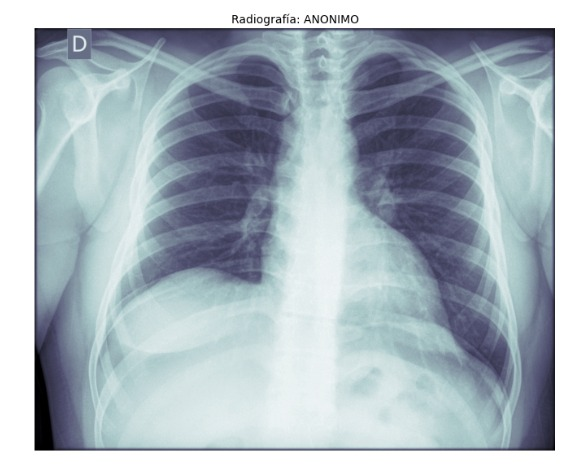
\includegraphics[width=\linewidth]{Tesis/radiografia_ok.jpeg}
    \end{minipage}
    \hfill
    \begin{minipage}[b]{0.48\textwidth}
        \small
        \textbf{Informe clínico asociado:}
        \vspace{0.3em}
        
        \textit{TÓRAX}
        
        No se observan procesos parenquimatosos activos.
        
        S.C.V. compatible con la edad.
        
        Domo diafragmático derecho conservado.
    \end{minipage}
    \caption{Ejemplo de una radiografía de tórax en formato DICOM junto a su informe radiológico correspondiente en la base de datos local.}
    \label{fig:ejemplo_radiografia}
\end{figure}

\section{Curado y estandarización de reportes textuales}

Dado que la mayoría de los modelos de lenguaje y arquitecturas multimodales del estado del arte han sido preentrenados en idioma inglés, se procedió a traducir la totalidad de los informes clínicos mediante el módulo \texttt{GoogleTranslator} de la biblioteca de Python \texttt{deep\_translator}.

Aunque una proporción importante de los informes presentaba una estructura técnica homogénea, se detectó ruido sistemático compuesto por firmas médicas, números de matrícula profesional, fechas de emisión, encabezados genéricos y descripciones marginales de otras regiones anatómicas evaluadas en la misma sesión clínica. Para remover estos artefactos textuales que habrían sesgado las métricas de evaluación de lenguaje natural, se diseñó un algoritmo de limpieza y filtrado basado en expresiones regulares (\autoref{code:filtro}).


La aplicación de este procedimiento permitió homogeneizar el cuerpo textual de los informes. En la \autoref{tab:ejemplos_filtro} se ilustra el efecto del filtrado y la traducción sobre casos representativos.

\begin{table}[htbp]
    \centering
    \small
    \begin{tabular}{|p{7cm}|p{7.5cm}|}
        \hline
        \textbf{Texto original (Crudo en español)} & \textbf{Texto estandarizado (Curado en inglés)} \\ \hline
        TÓRAX \newline No se observan procesos parenquimatosos activos. \newline S.C.V. Compatible con la edad. \newline \newline RODILLA DERECHA \newline Signos de artrosis. Calcificaciones intra y periarticulares. & No active parenchymal processes are observed. S.C.V. compatible with age. \\ \hline
        TÓRAX \newline No se observan procesos parenquimatosos activos. \newline Aorta desenrollada. \newline \newline Dr. Xxxxx Xxxxxxx \newline MP. XXXX & No active parenchymal processes are observed. Aorta uncoiled. \\ \hline
    \end{tabular}
    \caption{Ejemplos del proceso de curado, remoción de ruido y traducción de informes radiológicos.}
    \label{tab:ejemplos_filtro}
\end{table}

\section{Agrupamiento semántico (Clustering) y balanceo del dataset}
\label{sec:clustering}

En tareas de aprendizaje automático aplicadas a la radiología, el balance de las clases dentro del conjunto de datos constituye un factor crítico. Un desbalance extremo dominado por estudios de rutina sin hallazgos patológicos puede inducir un sesgo en los modelos generativos y de clasificación, afectando negativamente su capacidad para identificar anomalías poco frecuentes.

Para caracterizar cuantitativamente la distribución diagnóstica de la población de $6\,123$ informes, se implementó una estrategia de agrupamiento semántico. En primer lugar, se generaron representaciones vectoriales densas (\textit{embeddings}) utilizando el modelo preentrenado \texttt{SentenceTransformers} (variante \texttt{all-MiniLM-L6-v2}), procesando los textos en lotes (\textit{batches}) de 32 muestras para optimizar la memoria (\autoref{code:clustering_embeddings}).



Posteriormente, sobre el espacio vectorial generado, se aplicó el algoritmo de agrupamiento basado en densidad DBSCAN (\textit{Density-Based Spatial Clustering of Applications with Noise}) \citep{3001460.3001507}. Se utilizó la distancia coseno como métrica de similitud con un radio de vecindad $\epsilon = 0.04$ y un umbral mínimo de 2 muestras por grupo (\texttt{min\_samples = 2}), según se muestra en el \autoref{code:clustering}.


El algoritmo identificó 100 clústeres semánticos diferenciados. El análisis cualitativo reveló que la distribución estaba severamente sesgada: un único clúster acumulaba más del $50\%$ de la población total de reportes (\autoref{fig:torta}). Dicho grupo estaba compuesto por informes de rutina con patrones textuales virtualmente idénticos (p. ej., \textit{``No active parenchymal processes are observed...''}). Asimismo, 435 informes permanecieron como ruido o puntos aislados (etiqueta $-1$) debido a la singularidad de sus descripciones patológicas.

\begin{figure}[htbp]
    \centering
    \begin{minipage}[b]{0.65\textwidth}
        \centering
        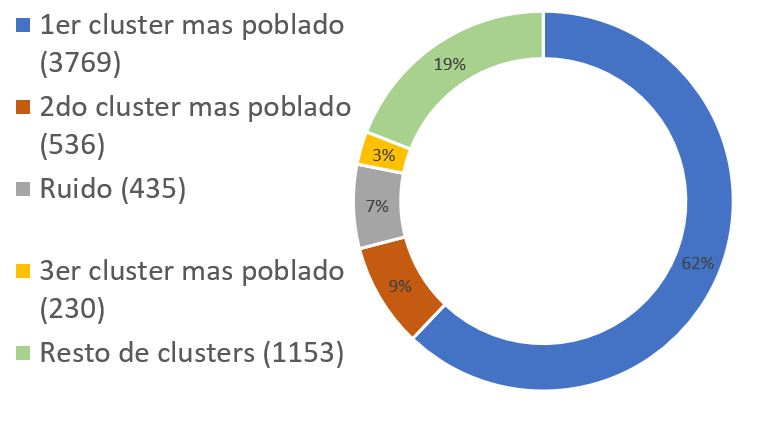
\includegraphics[width=\linewidth]{Tesis/Torta clusters.png}
    \end{minipage}
    \hfill
    \begin{minipage}[b]{0.30\textwidth}
        \small
        \textbf{Informe típico del clúster dominante:}
        \vspace{0.3em}
        
        \textit{TÓRAX}
        
        No se observan procesos parenquimatosos activos.
        
        S.C.V. compatible con la edad.
    \end{minipage}
    \caption{Distribución de la población de informes en clústeres semánticos mediante DBSCAN y patrón textual del grupo mayoritario.}
    \label{fig:torta}
\end{figure}

Para mitigar este desbalance y evitar la sobre-representación de estudios normales durante la evaluación, se estableció un límite superior estricto de 500 expedientes para cualquier clúster. Tras aplicar esta subsimplificación (\textit{undersampling}) dirigida sobre el grupo mayoritario, el dataset balanceado se consolidó en $2\,818$ expedientes (asociados a $4\,289$ radiografías).

\section{Censo de imágenes y metadatos radiológicos}
\label{sec:censo_metadatos}

A partir de las $4\,289$ radiografías contenidas en los $2\,818$ expedientes balanceados, se realizó un censo descriptivo utilizando los metadatos almacenados en las cabeceras DICOM. Se constató que el $100\%$ de los archivos disponía de información relativa a la proyección radiográfica, el $98.97\%$ registraba el sexo del paciente y el $17.21\%$ incluía la edad. No se identificaron campos estructurados referentes a síntomas o motivos explícitos de consulta ni historial clínico.

\begin{figure}[htbp]
    \centering
    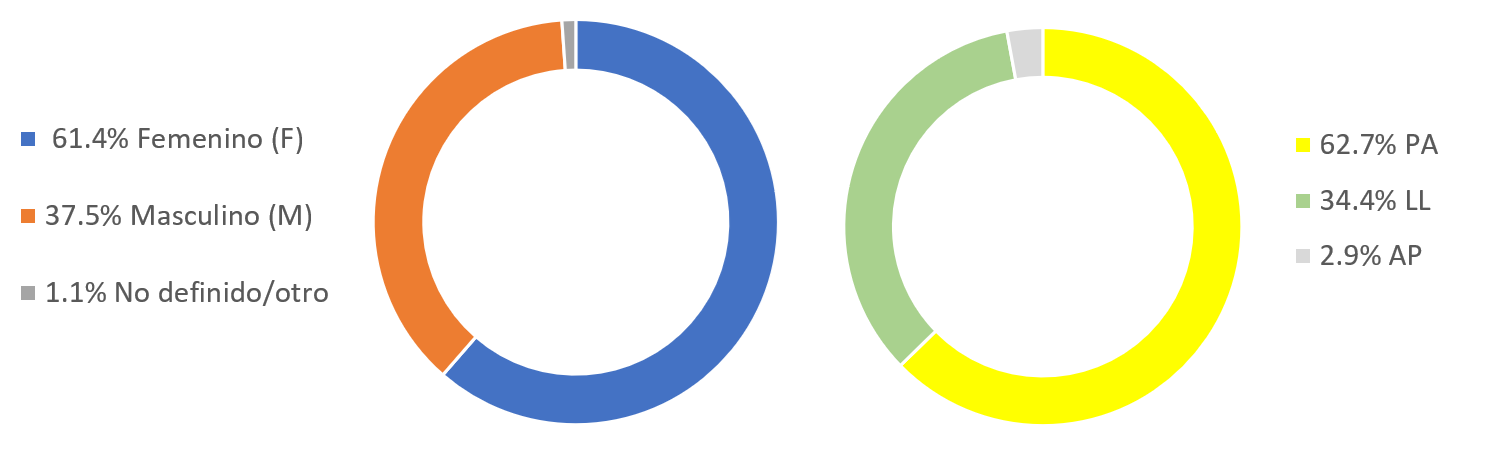
\includegraphics[width=1\textwidth]{Tesis/Torta vistas.png}
    \caption{Distribución demográfica y de proyecciones radiográficas en el dataset balanceado.}
    \label{fig:tortas_radiografias}
\end{figure}

La distribución por sexo arrojó un $61.41\%$ de pacientes de sexo femenino (F), un $37.47\%$ de sexo masculino (M) y un $1.12\%$ sin especificar. Respecto a las proyecciones anatómicas, predominó la vista Posteroanterior (PA) con un $62.74\%$, seguida por la Laterolateral (LL) con un $34.39\%$ y la Anteroposterior (AP) con un $2.87\%$ (\autoref{fig:tortas_radiografias}).

En cuanto al equipamiento, el $100\%$ de las capturas fue realizado con tecnología de la marca AGFA, correspondiendo el $99.02\%$ al modelo \texttt{DXD40\_1000G} y el $0.98\%$ al modelo \texttt{CR 35}.

El análisis de la resolución radiométrica reveló que el $85.3\%$ de los archivos poseía una profundidad de $8$ bits, mientras que el $14.7\%$ presentaba $12$ bits. La correlación con las fechas de adquisición indicó que las imágenes de 12 bits fueron capturadas entre agosto de 2021 y marzo de 2022, mientras que las de 8 bits corresponden al período entre marzo de 2022 y enero de 2026. Dado que el hardware no sufrió modificaciones, esta variación se atribuye a un cambio en el procesamiento de software interno del centro médico.

Por último, el tamaño espacial de las imágenes mostró variaciones según la proyección: la vista PA presentó una resolución promedio de $2456 \times 2641$ píxeles; la vista LL, de $2735 \times 2163$ píxeles; y la vista AP, de $1730 \times 1844$ píxeles. Cabe destacar que las heterogeneidades de profundidad de bit y dimensiones espaciales identificadas en este censo justificaron el diseño de la etapa de preprocesamiento unificado (escalado dinámico de ventana, CLAHE y redimensionamiento a $512 \times 512$ píxeles) descrito en la \autoref{sec:Preprocesamiento, Carga y Estandarización de Datos}.

\section{Consideraciones éticas, privacidad y gobernanza de datos}
\label{sec:consideraciones_eticas}

El desarrollo de este trabajo se rigió por estrictos estándares de ética, privacidad y gobernanza de datos aplicados a la investigación retrospectiva en salud. El conjunto de datos radiológicos utilizado provino de un repositorio institucional anonimizado (Instituto Lavalle 11 de Bahía Blanca). Con el propósito de resguardar la confidencialidad y cumplir con la normativa de protección de datos en el ámbito médico, todas las cabeceras de los archivos DICOM fueron depuradas de forma previa, eliminando cualquier metadato de identificación personal (tales como nombres, números de documento o datos de afiliación directa del paciente). 

Asimismo, al tratarse de un estudio retrospectivo basado en registros históricos sin intervención directa sobre los sujetos ni alteración de los protocolos clínicos asistenciales, se garantizó el resguardo absoluto de la anonimidad y la integridad ética en el procesamiento secundario de las imágenes y los informes.


\end{document}